% Chapter 1

\chapter{Introduction} % Write in your own chapter title
\label{Chapter1}

Many analytical and empirical relations have been derived to model fluid motion under simplifying assumptions, but there are many applications of great engineering interest that are too complicated to be modeled by these simple relations. The field of computational fluid dynamics (CFD) has arisen to allow engineers to model and understand more complicated systems. The majority of familiar CFD codes describe fluid motion from an Eulerian perspective in which the fluid moves through a stationary grid, and fluid properties such as density, energy, and velocity are calculated based on flux through cell boundaries. Eulerian CFD \cite{Tannehill1997} is most appropriate when the domain of the problem is unchanging. Some common applications of Eulerian CFD include external flow over a wing or whole aircraft \cite{AircraftCFD}, pipe and duct flow \cite{DuctCFD}, ground vehicle aerodynamics \cite{Perry2008}, convective heat transfer for electronics \cite{ElectronicsCFD}, or even process modeling \cite{SugarCFD}, and ship design \cite{ShipCFD}.

A less common, but equally valid description, is the Lagrangian framework of fluid motion. In Lagrangian CFD codes, the mesh moves in time with the material. This is especially appropriate in cases where the problem domain itself is changing as is the case with many unsteady simulations. The area where Lagrangian methods particularly shine is in multi-material simulations and interface tracking. Applications include free surface flow \cite{FreeSurfaceCFD, FreeSurfaceCFD2}, detonations \cite{ExplosionCFD}, astrodynamics \cite{AstroCFD}, fluid-structure interaction \cite{FluidStructureCFD}, and even full simulations of nuclear tests. 

A popular flavor of CFD codes solve the Euler equations, often in a Lagrangian frame, and are commonly known as hydrocodes \cite{HydroCodeBook}. The Euler equations are derived by taking the full Navier-Stokes equations and assuming that inertial forces are much more significant than viscous forces. This eliminates all viscous terms and reduces the equations down to a set of simple PDE's for mass, momentum, and energy conservation. The desired unknowns are density, velocity, and energy, from which we can derive any additional thermodynamic terms such as pressure. 

Lagrangian simulations have been deemed more ``delicate'' because what may have been an initially sound mesh may become self-intersecting as the solution progresses. Complicated or vortical flows can often cause Lagrangian meshes to tangle. In these cases, the fluid moves in such a way that the mesh cannot follow and the mesh vertices start to tangle resulting in non-physical predictions like negative density or pressure. One technique that has arisen to address this issue is the Arbitrary Lagrangian Eulerian \cite{DonaeALE} (ALE) technique. The Lagrange step \cite{Tipton90} is still at the heart of this method, but when mesh tangling is sensed, the fluid motion simulation is paused as the mesh is relaxed to a less tangled state. During the mesh relaxation stage, all of the stationary state variables are conservatively advected through the moving mesh, monotonically if possible. Then the fluid simulation resumes with this less tangled mesh until the mesh begins to tangle again.

Most ALE CFD codes use a Staggered Grid Hydrodynamics \cite{Burton1994} (SGH) scheme in which thermodynamic variables like energy, density, and pressure are defined at cell centers and kinematic variables like position and velocity are defined at cell nodes. Traditionally ALE staggered grid hydrocodes have used low order elements such that for quadrilaterals, thermodynamic variables are interpolated as constant within each cell but discontinuous between cells, and kinematic variables are interpolated bi-linearly within a cell and are continuous between adjacent cells.

While traditional SGH codes have been successful in many applications, their predictive capability can be limited by several long-standing issues. Notable among these are symmetry preservation, energy conservation, the artificial viscosity discretization, and hourglass mode instabilities, see \refFig{HGExample} and \refFig{Noh_SymmetryBreak}. This research seeks high-order finite element solutions to these problems. In particular we develop a method that is energy conserving by design with a tensor artificial viscosity formulation, and high order kinematic and thermodynamic representations.
% The overarching goal of our finite element hydrocode research group at Lawrence Livermore National Laboratory is to address these issues by developing modern finite element discretization schemes using high-order, multi-scale and discontinuous Galerkin methods. 
% The research presented in this thesis considered whether high-order finite element discretizations are even feasible for shock hydrodynamics simulations.

\begin{figure}[h!]
 \centering
 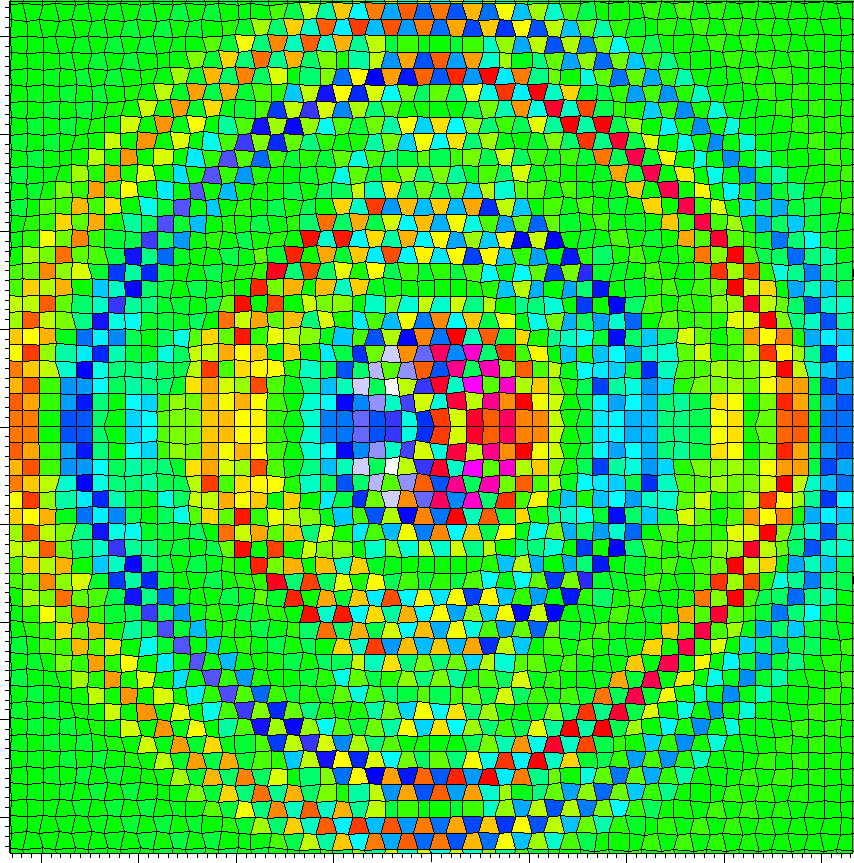
\includegraphics[width=4in,keepaspectratio=true]{./Figures/HGExample.png}
 % gradpField.png: 871x527 pixel, 90dpi, 24.59x14.88 cm, bb=0 0 697 422
 \caption{Example of a “checkerboard” instability in the pressure field and corresponding “hourglass” instability in velocity field; excited by applying a time dependent perturbation to a single node at the center. Instability exists at highest spatial frequency of the underlying grid irrespective
of mesh resolution and is a result of a fundamental instability in the discrete representation of velocity, pressure and the spatial differential operators which relate them.}
 \label{fig:HGExample}
\end{figure}

\begin{figure}[h!]
 \centering
 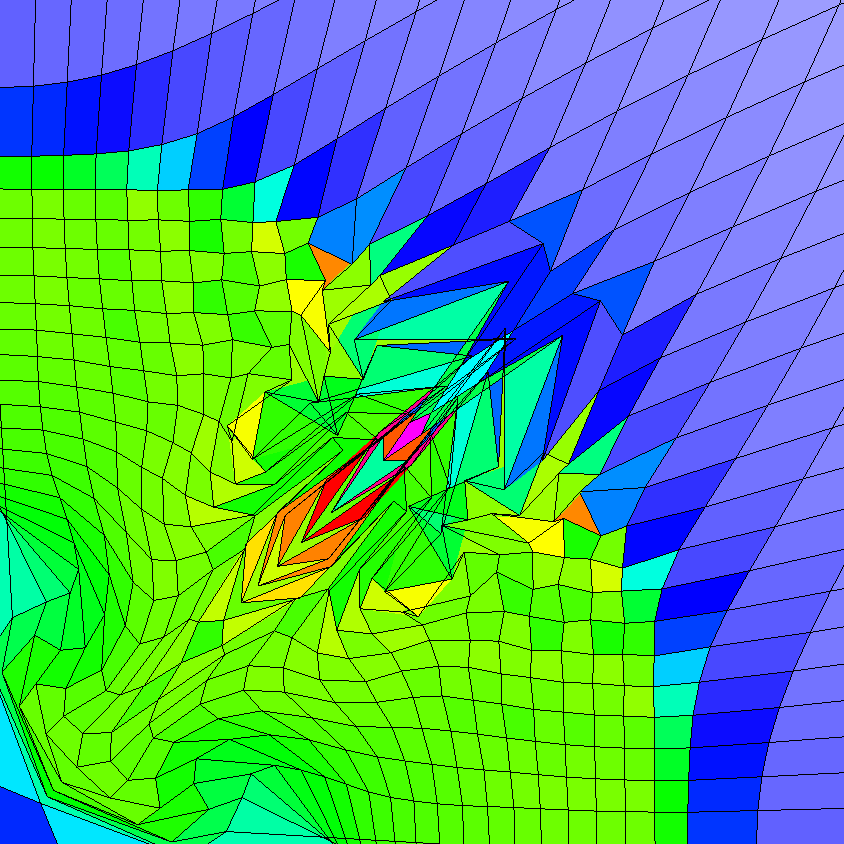
\includegraphics[width=4in,keepaspectratio=true]{./Figures/Noh_SymmetryBreak.png}
 % gradpField.png: 871x527 pixel, 90dpi, 24.59x14.88 cm, bb=0 0 697 422
 \caption{Example of spurious grid distortion encountered when applying standard SGH methods to the Noh problem on an initially orthogonal mesh. There are multiple sources of this grid distortion including hourglass instabilities, inaccuracies in the pressure gradient operator and discretization of the artificial viscosity term. Each of these errors can amplify each other over time, leading to a rapid tangling of the grid.}
 \label{fig:Noh_SymmetryBreak}
\end{figure}

A high order finite element test-bed has been developed in Matlab to evaluate the potential of high order finite elements for Lagrangian hydrodynamics. Several test problems will be considered to assess the usefulness of such methods. A set of static convergence tests will measure and compare the convergence rates of several methods. A significant concern with any new method is the presence of spurious velocity and pressure modes; this will be observed through the acoustic wave problem. The Sod shock tube will evaluate the one-dimensional convergence to the exact solution of a real time-evolving solution, while the Noh problem will bring this evaluation to two dimensions. The Saltzman piston will measure how conducive each method is to propagating a shock wave that is misaligned with the mesh, this will primarily be a test of the artificial viscosity formulation. Finally, the Sedov explosion problem will compare the adaptivity of low and high order methods to curved phenomena. The biggest worry when considering any higher order numerical method is high-frequency ``ringing'' about the shock front. The severity (or not) of this property will be noted as it comes up.

Chapter 2 of this thesis will develop a theoretical framework for arbitrarily high order finite element schemes for Lagrangian hydrodynamics, while Chapter 3 will consider the implementation details in the \texttt{Fermium} code. Chapter 4 narrows the problem domain from a wide range of bi-linear and bi-quadratic elements to four mixed finite element pairs which bear further consideration. Numerical results for each of these methods are presented in Chapter 5 and conclusions are drawn in Chapter 6.